\documentclass[12pt,a4paper,titlepage]{article}
\usepackage[utf8]{inputenc}
\usepackage[finnish]{babel}
\usepackage{setspace}
\usepackage{parskip}
\usepackage{amssymb}
\usepackage{amsmath}
\usepackage{graphicx}
\usepackage{fancyhdr}
\usepackage[top=1in, bottom=1in, left=1in, right=1in]{geometry}
\usepackage{float}
\usepackage[section]{placeins}
%\usepackage[numbered,autolinebreaks,useliterate]{mcode} % jos tahdot laittaa matlabkoodia näkyville niin kannattaa käyttää tätä

% hyödyllisiä paketteja:
\usepackage{siunitx}\sisetup{per=frac} % SI-yksiköitä.
%\usepackage{supertabular} % jos tarttee isoja taulukoita
%\usepackage{fullpage} % pienemmät marginaalit jos haluaa

\usepackage{hyperref} % lisääthän omat pakettisi ENNEN hyperref'iä
\hypersetup{pdfborder={0 0 0}}
\onehalfspacing
\cfoot{}
\rhead{\thepage}
% asettaa nyk. kappaleen nimen vasempaan ylänurkkaan, saa poistaa jos haluaa
\lhead{\leftmark}

\newcommand{\matr}[1]{\mathbf{#1}}

%%%%% kaikki ennen tätä liittyy käytettäviin paketteihin tai dokumentin muotoiluun. siihen ei tarvinne aluksi koskea. %%%%%

%%%%% kansilehti %%%%%
\title{Taivaanmekaniikka \\ Lineaarinen pienimmän neliösumman sovitus \vspace{0.5em}}
\author{\begin{tabular}{c}
Anni Järvenpää
\end{tabular}}
\date{\today}
\begin{document}
\maketitle

%%%%%%%%%%%%%%% Oleellinen sisältö alkaa%%%%%%%%%%%%%%%
\section{Lineaarinen pienimmän neliösumman menetelmä}
Lineaarisen pienimmän neliösumman menetelmän tavoitteena on sovittaa pisteistä $(x_i, y_i)$ koostuvaan havaintoaineistoon suora, joka edustaa pisteitä mahdollisimman hyvin. Tyypillisesti sovituksen hyvyyttä mitataan pisteiden vertikaalisena etäisyytenä sovitetusta suorasta (merkitty sinisellä kuvassa \ref{vertikaalietaisyys}). Pienimmän neliösumman menetelmässä näiden vertikaalisten poikkeamien neliöiden summa pyritään minimoimaan, siis etsimään funktion $f(x) = kx+b$ kertoimet $k$ ja $b$ siten, että virhe $S$ on mahdollisimman pieni, kun $S$ on määritelty seuraavasti:
\begin{equation}
	S=\sum\limits_{i=1}^{n} (y_i - f(x_i))^2
\end{equation}

\begin{figure}
\centering
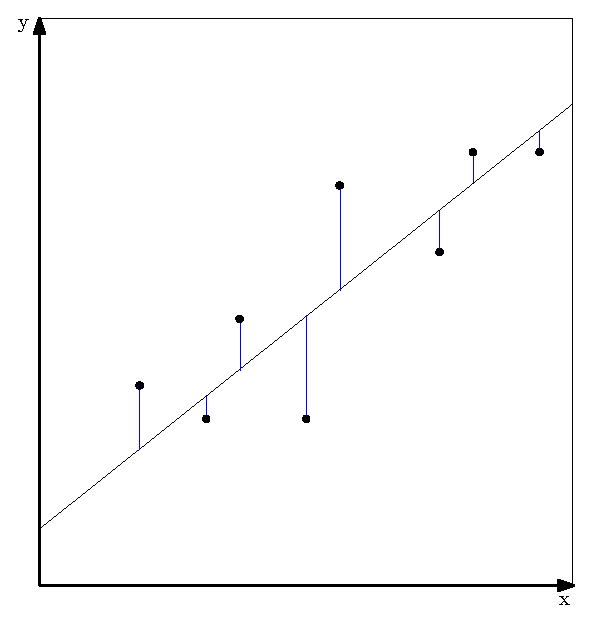
\includegraphics{vertikaalietaisyys.eps} %lveydeksi voi antaa myös vaikkapa 5cm tai muun konkreettisen mitan tai vaihtoehtoisesti asettaa leveydeksi vaikapa 80% tekstin leveydestä parametrilla 0.8\textwidth. Kuvan korjeuden voi asettaa esimerkiksi height=6cm.
\caption{Pistejoukko, johon sovitettu suora mustalla ja pisteiden vertikaaliset etäisyydet suorasta pisteinä.}
\label{vertikaalietaisyys}
\end{figure}

Mikäli havaintopisteitä on vain kaksi tai pisteet ovat täsmälleen suoralla, voidaan 

%Matriisimuodossa tämä voidaan kirjoittaa
%\begin{equation}
%	\matr{Y} = \matr{\Phi}\matr{\Theta} + \matr{E},
%\end{equation}
%missä $\matr{Y}$ ja $\matr{E}$ ovat $n$ mittaisia vektoreita, $\matr{\Theta}$ on $p$ mittainen vektori, missä $p$ on vapaiden parametrien määrä, ja $\matr{\Phi}$ on ($n \times p$) matriisi. 

%%%%% Sisältö loppuu, lähdeluettelo %%%%%
\bibliographystyle{plain}
\bibliography{lahteet} 
\appendix
\newpage
\section{Liittyvä liite.} \label{koodi}
Liian laaja leipätekstiin.
\end{document}
